\section{Benutzerinteraktion}
Die Benutzerinteraktion wurde sehr übersichtlich gestaltet, um den Client eine m\"oglichst kompakte, intuitive Bedienbarkeit zur Verfügung zu stellen. F\"ur den Anwender wurde deshalb eine Schnittstelle mit dem MBean Server kreiert (Siehe dazu Abschnitt \ref{controller}), welche ausschlie\ss lich vier unterschiedliche Funktionalitäten anbietet. \\
In Abbildung \ref{AnFallDia} ist diese Benutzerinteraktion als Anwendungsfalldiagramm bzw. Nutzfalldiagramm dargestellt. Die ersten beiden Operationen der Anwendung mit ähnlicher Funktionalität, geben alle Fehlerwerte respektive die ID's der annotierten Streams zurück. Dies ist insbesondere von Vorteil, wenn später die Fehlerwerte geändert werden sollen und die eindeutige ID des Streams nicht bekannt ist. \\
Um die Fehlerwerte der einzelnen Streams ändern zu können, gibt es eine Methode die in Abbildung \ref{AnFallDia} unter ``Fehlerwerte \"andern'' zu finden ist. Die Änderungsmöglichkeiten umfassen die Fehlerrate, Fehlertyp und die grö\ss e des Datenblocks. Die ID dient zur Zuordnung der Fehlerwerte und kann ausschlie\ss lich im Programmcode ver\"andert werden.\\
Die wichtigste Funktion hat den Namen \courier{runInjection} und ist in Abbildung \ref{AnFallDia} als ``Injektion durchführen'' dargestellt. Für diese Funktion lassen sich zwei Varianten auswählen. Die erste Variante ist für eine Dateiinjektion definiert und benötigt lediglich den Dateipfad. Die zweite Variante verlangt einen Java \courier{InputStream} um allgemeine Datenströme zu verarbeiten. Nach dem Laden der Daten wird durch diese Funktion die eigentliche Fehlerinjektion und die Datenausgabe veranlasst.\\
Für die Datenausgabe sind ebenfalls zwei Wahlmöglichkeiten vorhanden, deren genaue Differenzierung im weiteren Verlauf dieses Kapitels erläutert wird.

\begin{figure}[!htb]
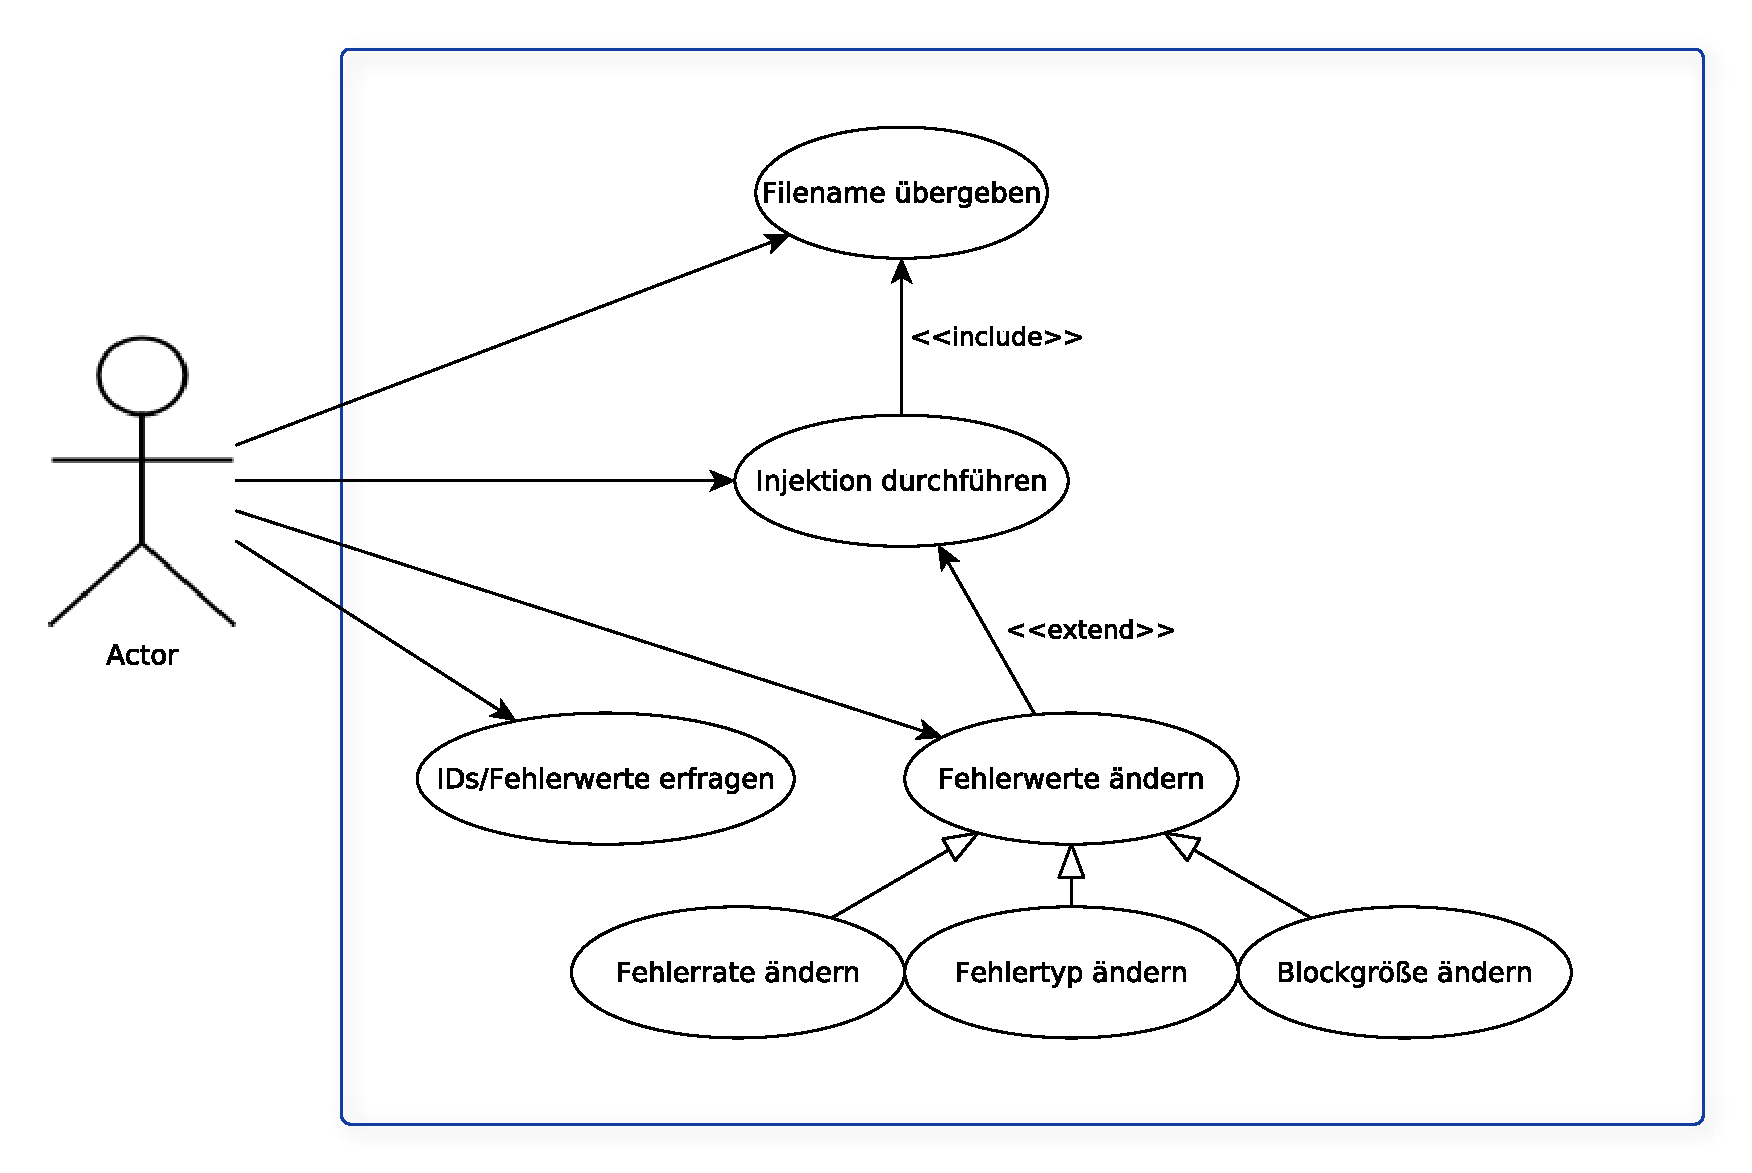
\includegraphics[scale=0.55]{graphics/Anwendungsfalldiagramm.eps}
\centering
 \caption[Anwendungsfalldiagramm]{Anwendungsfalldiagramm}
 \label{AnFallDia}
\end{figure}
